\documentclass[11pt]{article}

\usepackage{latexsym,amsmath,array,dcolumn}
\usepackage[utf8]{inputenc}
\usepackage[version=4]{mhchem}
\usepackage{graphicx}
\usepackage{wrapfig}
\usepackage{epsfig}
\usepackage{epstopdf}
\usepackage{caption}
\usepackage{textcomp}
\usepackage{xfrac}
\usepackage{pbox}
\usepackage{gensymb}
\usepackage[labelfont=bf,]{caption}
\usepackage[sort&compress,numbers,super]{natbib}
\usepackage{hyperref}
\hypersetup{colorlinks=true, linkcolor=blue, citecolor=blue}
\usepackage[capitalize]{cleveref}
\usepackage{gensymb}
\usepackage{textcomp}
\usepackage{bpchem}
\usepackage{pifont}
\usepackage{booktabs}
\usepackage{xspace}
\usepackage{float}
\usepackage{multirow}
\usepackage{braket}
\usepackage{authblk}
\usepackage{bm}
\usepackage{rotating}
\usepackage{wallpaper}
\usepackage{ragged2e}
\usepackage{tikz}
\usepackage{stackengine}
\usepackage{titlesec}
\usepackage{mathpazo}
\usepackage[left=2.5cm,right=2.5cm,top=2.5cm,bottom=3cm]{geometry}
\usepackage{mathtools}
\usepackage{listings}
\usepackage{courier}
\usepackage{enumitem}

\titleformat*{\section}{\large\bfseries}
\renewcommand{\baselinestretch}{1.5}

\renewcommand{\figurename}{Fig.}

\definecolor{bash}{rgb}{0.80,0.80,0.80}

% macros
\newcommand{\todo}[1]{\textcolor{red}{#1}\xspace}

\lstset{ 
  backgroundcolor=\color{lightgray!20!white}
}
\lstset{basicstyle=\ttfamily,breaklines=true,xleftmargin=30pt}

\title{rhOver}
\author{Michael B\"{o}hme}
\date{User Manual}

\begin{document}

\pagestyle{empty}

\begin{center}
 
 \vspace*{180pt}
 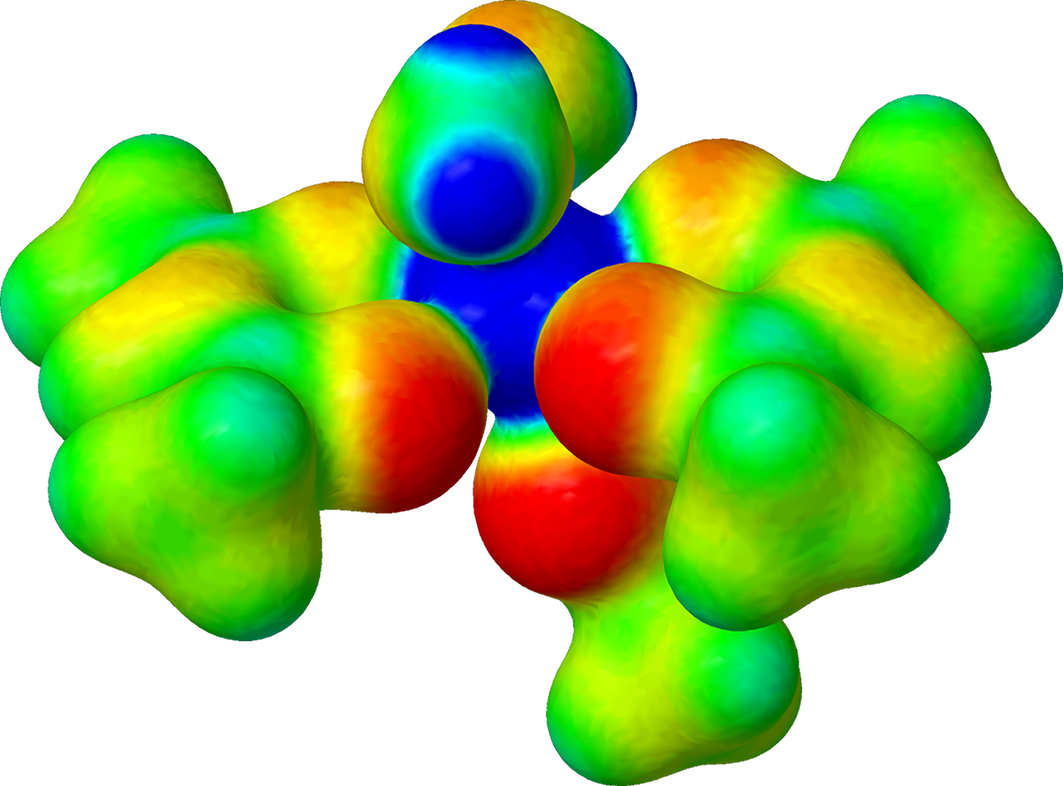
\includegraphics[width=6cm]{DEPP} \\[10pt]
 
 \Huge{\bfseries rhOver} \\[20pt]
 \normalsize
 User Manual \\
 v1.00 \\[45pt]
 A FORTRAN Program to Determine Magnetic Anisotropy and Related Properties for Dysprosium(\textsc{iii}) Single-Ion Magnets by Semi-Empirical Approaches utilizing Hartree--Fock \mbox{Wave Functions} \\[25pt]
  
 Copyright \textcopyright~2014--2019 Michael Böhme \\
 This document is part of \texttt{rhOver}. \\ 
 By downloading and/or using this software you agree to the terms of its license.
\end{center}

\clearpage
\pagestyle{plain}

\tableofcontents
	
\clearpage
\section{Introduction to rhOver}

\subsection{What is rhOver?}

\clearpage
\subsection{License}

\texttt{rhOver} is released under the MIT license. \\

\noindent
Copyright \textcopyright~2014--2019 Michael Böhme \\

\noindent
Permission is hereby granted, free of charge, to any person obtaining a copy
of this software and associated documentation files (the "Software"), to deal
in the Software without restriction, including without limitation the rights
to use, copy, modify, merge, publish, distribute, sublicense, and/or sell
copies of the Software, and to permit persons to whom the Software is
furnished to do so, subject to the following conditions: \\

\noindent
The above copyright notice and this permission notice shall be included in all
copies or substantial portions of the Software. \\

\noindent
THE SOFTWARE IS PROVIDED "AS IS", WITHOUT WARRANTY OF ANY KIND, EXPRESS OR
IMPLIED, INCLUDING BUT NOT LIMITED TO THE WARRANTIES OF MERCHANTABILITY,
FITNESS FOR A PARTICULAR PURPOSE AND NONINFRINGEMENT. IN NO EVENT SHALL THE
AUTHORS OR COPYRIGHT HOLDERS BE LIABLE FOR ANY CLAIM, DAMAGES OR OTHER
LIABILITY, WHETHER IN AN ACTION OF CONTRACT, TORT OR OTHERWISE, ARISING FROM,
OUT OF OR IN CONNECTION WITH THE SOFTWARE OR THE USE OR OTHER DEALINGS IN THE
SOFTWARE. 

\clearpage
\subsection{Citation for rhOver}

Please quote the usage of the \texttt{rhOver} program and any scientific results in any form obtained with it by the following reference:

\begin{itemize}
 \item \textbf{rhOver: Determination of Magnetic Anisotropy and Related Properties for Dysprosium(\textsc{iii}) Single-Ion Magnets by Semi-Empirical Approaches utilizing Hartree--Fock Wave Functions.} Michael Böhme, Winfried Plass, \textit{J. Comput. Chem.} \textbf{2018}, \emph{39} (32), 2697--2712.
\end{itemize}

\clearpage
\section{Installation Guide}

\texttt{rhOver} is distributed as FORTRAN source code and needs to be compiled in order to use the program.

\noindent
\paragraph{Please note:} Currently, \texttt{rhOver} only supports MOLDEN files which have been generated by TURBOMOLE.\cite{TURBOMOLE}
However, the support of other quantum computational software is planned for future releases of \texttt{rhOver}.
If you or your institution did not obtain a valid TURBOMOLE license, you can \href{http://www.cosmologic.de/support-download/downloads/turbomoledemolicenseagreement.html}{apply} for a limited demo version of TURBOMOLE.
Furthermore, it is recommended to install additional scalar-relativistic optimized basis sets (see section \ref{sec:tmbasis} \nameref{sec:tmbasis}).

\subsection{Prerequisites}

The following programs and software packages are required to compile \texttt{rhOver}:

\begin{itemize}
 \item a 64-bit FORTRAN compiler (with support for FORTRAN95 or later)
 \item GNU make
 \item BLAS development files and libraries
 \item LAPACK development files and libraries
\end{itemize}

\noindent
\texttt{rhOver} was successfully tested with the following FORTRAN compilers:

\begin{itemize}
 \item GNU Fortran (\texttt{gfortran})
 \item Intel \textregistered~ Fortran Compiler (\texttt{ifort})
\end{itemize}

\noindent
Please use your package management software of your Linux distribution to install the necessary BLAS and LAPACK development files and libraries.

\subsection{Building rhOver}\label{sec:building}

\begin{lstlisting}[frame=single,backgroundcolor=\color{bash}]
 tar xzf rhOver_v1.00.tar.gz
 cd rhOver/
\end{lstlisting}

\begin{lstlisting}[frame=single,backgroundcolor=\color{bash}]
 make -f Makefiles/TARGET
\end{lstlisting}

\begin{table}[h!]
 \centering
 \caption{Available targets for building \texttt{rhOver}}
 \label{tab:targets}
  \begin{tabular}{ll}
   \toprule
    \texttt{TARGET}          & description \\
   \midrule
    \texttt{gfortran-omp}    & GNU gfortran with OpenMP parallelization \\
    \texttt{gfortran-serial} & GNU gfortran \\
    \texttt{ifort-omp}       & Intel \textregistered~ Fortran Compiler with OpenMP parallelization \\
    \texttt{ifort-serial}    & Intel \textregistered~ Fortran Compiler \\
   \bottomrule
  \end{tabular}
\end{table}

\begin{lstlisting}[frame=single,backgroundcolor=\color{bash}]
 cp rhover $HOME/bin/
\end{lstlisting}

\subsection{Running rhOver}

\begin{lstlisting}[frame=single,backgroundcolor=\color{bash}]
 $HOME/bin/rhover input.dy3 > output.log &
\end{lstlisting}

\subsection{Installation of Recommended Basis Sets for Turbomole}\label{sec:tmbasis}

For all calculations we strongly recommend the usage of the scalar-relativistic basis sets DZP-DKH/TZP-DKH\cite{Jorge2009} and SARC-DKH.\cite{Pantazis2009}
These basis sets have been successfully tested in the original publication.\cite{rhOver} 
Unfortunately, these basis sets are not redistributed in the default TURBOMOLE installation and thus, have to be installed manually. 
The usage of other basis sets than the tested ones especially smaller basis sets is not recommended. 

\paragraph{Please note:} For all calculations all-electron GTO basis sets must be used, since \texttt{rhOver} does not support effective core potentials (ECPs). \\

\noindent
The DZP-DKH/TZP-DKH\cite{Jorge2009} and SARC-DKH\cite{Pantazis2009} basis sets are provided within the distribution files of \texttt{rhOver} and can be found in the DKH-BS subfolder.
To install these basis sets for your TURBOMOLE installation edit or create a file called \texttildelow/.definerc in your home folder.
Add the following line stating the exact path to your \texttt{rhOver} installation:

\begin{lstlisting}[frame=single,backgroundcolor=\color{bash},emph={username,path_to_rhOver_installation},emphstyle={\itshape}]
 basis=/home/username/path_to_rhOver_installation/DKH-BS
\end{lstlisting} 

\noindent
To check if the installation of the new basis set library was successfully, start TURBOMOLE's \texttt{define}, load a structure, and type 'lib' at the 'ATOMIC ATTRIBUTE DEFINITION MENU'. The new basis set library should be listened there as in this example:

\begin{lstlisting}[frame=single,backgroundcolor=\color{bash}]
 AVAILABLE BASIS SET LIBRARIES:
    #1  /share/apps/TURBOMOLE-7.2/basen/
    #2  /share/apps/TURBOMOLE-7.2/basold/
    #3  /home/michael/rhOver/DKH-BS/
 INPUT NUMBER OF DESIRED LIBRARY (DEFAULT = 1)
\end{lstlisting}

\noindent
At this point, the new basis set library is selected by typing '3'. Subsequently, the basis sets can be assigned to the atoms by employing the 'b' command. Note that TURBOMOLE automatically assigns basis sets with ECPs for heavy atoms. After assigning the new all-electron basis sets (see Table \ref{tab:basis}) all assigned ECPs can be deleted by entering 'ecprm all'.

\begin{table}[h!]
 \centering
 \caption{Recommended basis sets for \texttt{rhOver}}
 \label{tab:basis}
  \begin{tabular}{lll}
   \toprule
    Atom                     & Basis set & Ref. \\
   \midrule
    Lu                       & SARC-DKH  & \cite{Pantazis2009} \\
    Y                        & TZP-DKH   & \cite{Jorge2009} \\
    all donor atoms          & TZP-DKH   & \cite{Jorge2009} \\
    non-donor atoms          & DZP-DKH   & \cite{Jorge2009} \\
   \bottomrule
  \end{tabular}
\end{table}

\clearpage
\section{User's Guide}

\subsection{Structure of a rhOver Input File}

\begin{lstlisting}[frame=single]
rhOver 
 ! This is a comment
 COMMAND
  Argument1 Argument2 Argument3 
End
\end{lstlisting}

\subsection{Basic Examples}

\subsection{Parallelization}

\texttt{rhOver} can take advantage of multi-processor CPUs and was programmed with OpenMP support. 
To use \texttt{rhOver} with parallelization it is necessary to build it with OpenMP support (\texttt{TARGET} must have been set to \texttt{gfortran-omp} or \texttt{ifort-omp}; see section \ref{sec:building} \nameref{sec:building})
By default the number of threads is set to the number of cores in your computer. The number of used threads can be adjusted by two different methods:

\begin{enumerate}[start=1]
 \item By setting/changing the following environment variable: 
\end{enumerate}

\begin{lstlisting}[frame=single,backgroundcolor=\color{bash}]
export OMP_NUM_THREADS=4
\end{lstlisting}

\begin{enumerate}[start=2]
 \item By adding the keyword \texttt{PARA} in the input file: 
\end{enumerate}

\begin{lstlisting}[frame=single]
PARA 
 4
\end{lstlisting}

\clearpage
\section{Advanced Examples}

\clearpage
\section{Keywords}

\subsection{ANGSTROM}

\paragraph{Description:} This command specifies that input coordinates, \emph{e.g.} by the keywords \texttt{DYIII} and \texttt{PCM}, are given units of \AA ngstr\"{o}m. By default input coordinates are given in atomic units. 

\paragraph{Usage:}~ 

\begin{lstlisting}[frame=single]
  ANGSTROM
\end{lstlisting}

\paragraph{Example:}~ 

\begin{lstlisting}[frame=single]
rhOver
! [...]
  ANGSTROM
  
  DYIII
   1.000 2.000 3.000
! [...]
End
\end{lstlisting}

\clearpage
\subsection{ATOMID}

\paragraph{Description:} This command specifies the central metal ion by the atom number as found in the MOLDEN file. This keyword is not available in PCM-mode and requires a MOLDEN file. In addition, this keyword cannot be used together with the \texttt{DYIII} keyword.

\paragraph{Usage:}~ 

\begin{lstlisting}[frame=single]
  ATOMID
   123
\end{lstlisting}

\paragraph{Example:}~ 

\begin{lstlisting}[frame=single]
rhOver
! [...]
  MOFILE
   input-file.molden
  
  ATOMID
   1
! [...]
End
\end{lstlisting}


\clearpage
\subsection{DANGLE}

\paragraph{Description:}~

\paragraph{Usage:}~ 

\begin{lstlisting}[frame=single]
  DANGLE
   5.0
\end{lstlisting}

\paragraph{Example:}~ 

\begin{lstlisting}[frame=single]
rhOver
! [...]

! [...]
End
\end{lstlisting}

\clearpage
\subsection{DELETE4F}

\paragraph{Description:}~This keyword deletes the 4f$^{14}$ contribution in the DEPP models \textbf{Lu} and \textbf{Lu--X} to obtain the altered DEPP models \textbf{Lu--B} and \textbf{Lu--BX}, respectively. This is achieved by deleting the corresponding contracted Gaussian-type orbitals.

\paragraph{Usage:}~ 

\begin{lstlisting}[frame=single]
  DELETE4F
\end{lstlisting}

\paragraph{Example:}~ 

\begin{lstlisting}[frame=single]
rhOver
! [...]
  MOFILE
   input-file.molden
  
  ATOMID
   1
  
  DELETE4F
! [...]
End
\end{lstlisting}

\clearpage
\subsection{DELETEALL}

\paragraph{Description:}~This keyword deletes any contribution from all electron shells of the central metal ion. This is achieved by deleting the corresponding contracted Gaussian-type orbitals. The usage of this keyword is \emph{not} recommended!

\paragraph{Usage:}~ 

\begin{lstlisting}[frame=single]
  DELETEALL
\end{lstlisting}

\paragraph{Example:}~ 

\begin{lstlisting}[frame=single]
rhOver
! [...]
  MOFILE
   input-file.molden
  
  ATOMID
   1
  
  DELETEALL
! [...]
End
\end{lstlisting}

\clearpage
\subsection{DYIII}

\paragraph{Description:} This command specifies the position of the central metal center by its Cartesian coordinates. By default input coordinates are given in atomic units. By additionally using the keyword `ANGSTROM` the input coordinates can be given in units of \AA ngstr\"{o}m. This keyword is not compatible with the \texttt{ATOMID} keyword.

\paragraph{Usage:}~ 

\begin{lstlisting}[frame=single]
  DYIII
   0.000 0.000 0.000
\end{lstlisting}

\paragraph{Example:}~ 

\begin{lstlisting}[frame=single]
rhOver
! [...]
  MOFile
   input-file.molden

  ANGSTROM
  
  DYIII
   1.000 2.000 3.000
! [...]
End
\end{lstlisting}

\clearpage
\subsection{END}

\paragraph{Description:}~This keyword defines the end of a \texttt{rhOver} input file. Everything behind that keyword gets ignored by the program.

\paragraph{Usage:}~ 

\begin{lstlisting}[frame=single]
  END
\end{lstlisting}

\paragraph{Example:}~ 

\begin{lstlisting}[frame=single]
rhOver
! [...]
End
\end{lstlisting}

\clearpage
\subsection{EXPERT}

\clearpage
\subsection{GRID}

\clearpage
\subsection{GRIDPRUNING / NOGRIDPRUNING}

\clearpage
\subsection{JOB}

\clearpage
\subsection{LDAX}

\clearpage
\subsection{LFTCUTOFF}

\clearpage
\subsection{LFTONLY}

\clearpage
\subsection{LINSCANRANGE}

\clearpage
\subsection{MAXGP}

\clearpage
\subsection{MAXITER}

\clearpage
\subsection{MJ}

\clearpage
\subsection{MOFILE}

\clearpage
\subsection{MULLIKEN}

\clearpage
\subsection{NODEPPFILE}

\clearpage
\subsection{NOLFT}

\clearpage
\subsection{NOSHIELDING}

\clearpage
\subsection{NOXYZ}

\clearpage
\subsection{OLFILE}

\clearpage
\subsection{PARA}

\clearpage
\subsection{PCM}

\clearpage
\subsection{PRINTBASIS}

\clearpage
\subsection{RADIALWF}

\clearpage
\subsection{RANDOMROT / NORANDOMROT}

\clearpage
\subsection{REFERENCE}

\clearpage
\subsection{SAVEGRIDPOINTS}

\clearpage
\subsection{SCALING}

\clearpage
\subsection{SCANINC}

\clearpage
\subsection{SCANRANGE}

\clearpage
\subsection{SETROT}

\clearpage
\subsection{SETROT3D}

\clearpage
\subsection{SHIELDING}

\clearpage
\subsection{TITLE}

\clearpage
\subsection{TRJFILE}

\clearpage
\subsection{VERBOSE}

\clearpage
% \section{References}

\bibliographystyle{angewchem}
\bibliography{Literature}

\end{document}

